\documentclass{article}
\usepackage[utf8]{inputenc}
\usepackage{natbib}
\usepackage{graphicx}
\usepackage{amsmath}


\title{Background Reading List Analysis}
\author{Robert Twyman}
\date{October 2018}

\maketitle


\begin{document}
I will write my notes regarding the first 5 documents that Kris sent me on October 8th 2018 in an email titled "RE:reading material"

The documents are \cite{Alessio2006}, \cite{Bailey2014}, \cite{Zeng2001}, \cite{vanderVos2017}, \cite{Qi2006}
\newpage

\tableofcontents

\newpage
\section{PET Image Reconstruction - 
alessioPETRecon} \cite{Alessio2006}
\subsection{The model}
One way to represent the imaging system is with the following linear relationship
\begin{equation}\label{eq.model}
p = Hf + n 
\end{equation} 
= Hf + n s the set of observations, H is the known system model, f is the unknown image, and n is the error in the observations. The goal of reconstruction is to use the data values p (projections through the unknown object) to find the image f.
\subsection{Central Slice Theorem}
also known as central-slice theorem or Fourier-slice theorem is a foundational relationship found in analytically image reconstruction. The theorem states that that the Fourier transform of a one-dimensional projection $p(s, \phi)$ is equivalent to a section, or profile, $P(v_s,\phi)$ at the same angle through the center of the two-dimensional Fourier transform of the object, Fig.\ref{Fig.Central-Slice}. Here we see that the 1D projection (photon detection in the "camera") is transformed into Fourier space. The Fourier projection is equivalent to a section/profile, at the same angle and through the center, of the 2D Fourier transform of the object. If we know $P(v_s,\phi)$ for all angles $0\leq \phi \leq \pi$ then we can fill in the values of $F(v_x,v_y)$. The inverse of this 2D Fourier transform provides us with $f(x,y)$ in the patient (lab) frame.

\begin{figure}
\centering
	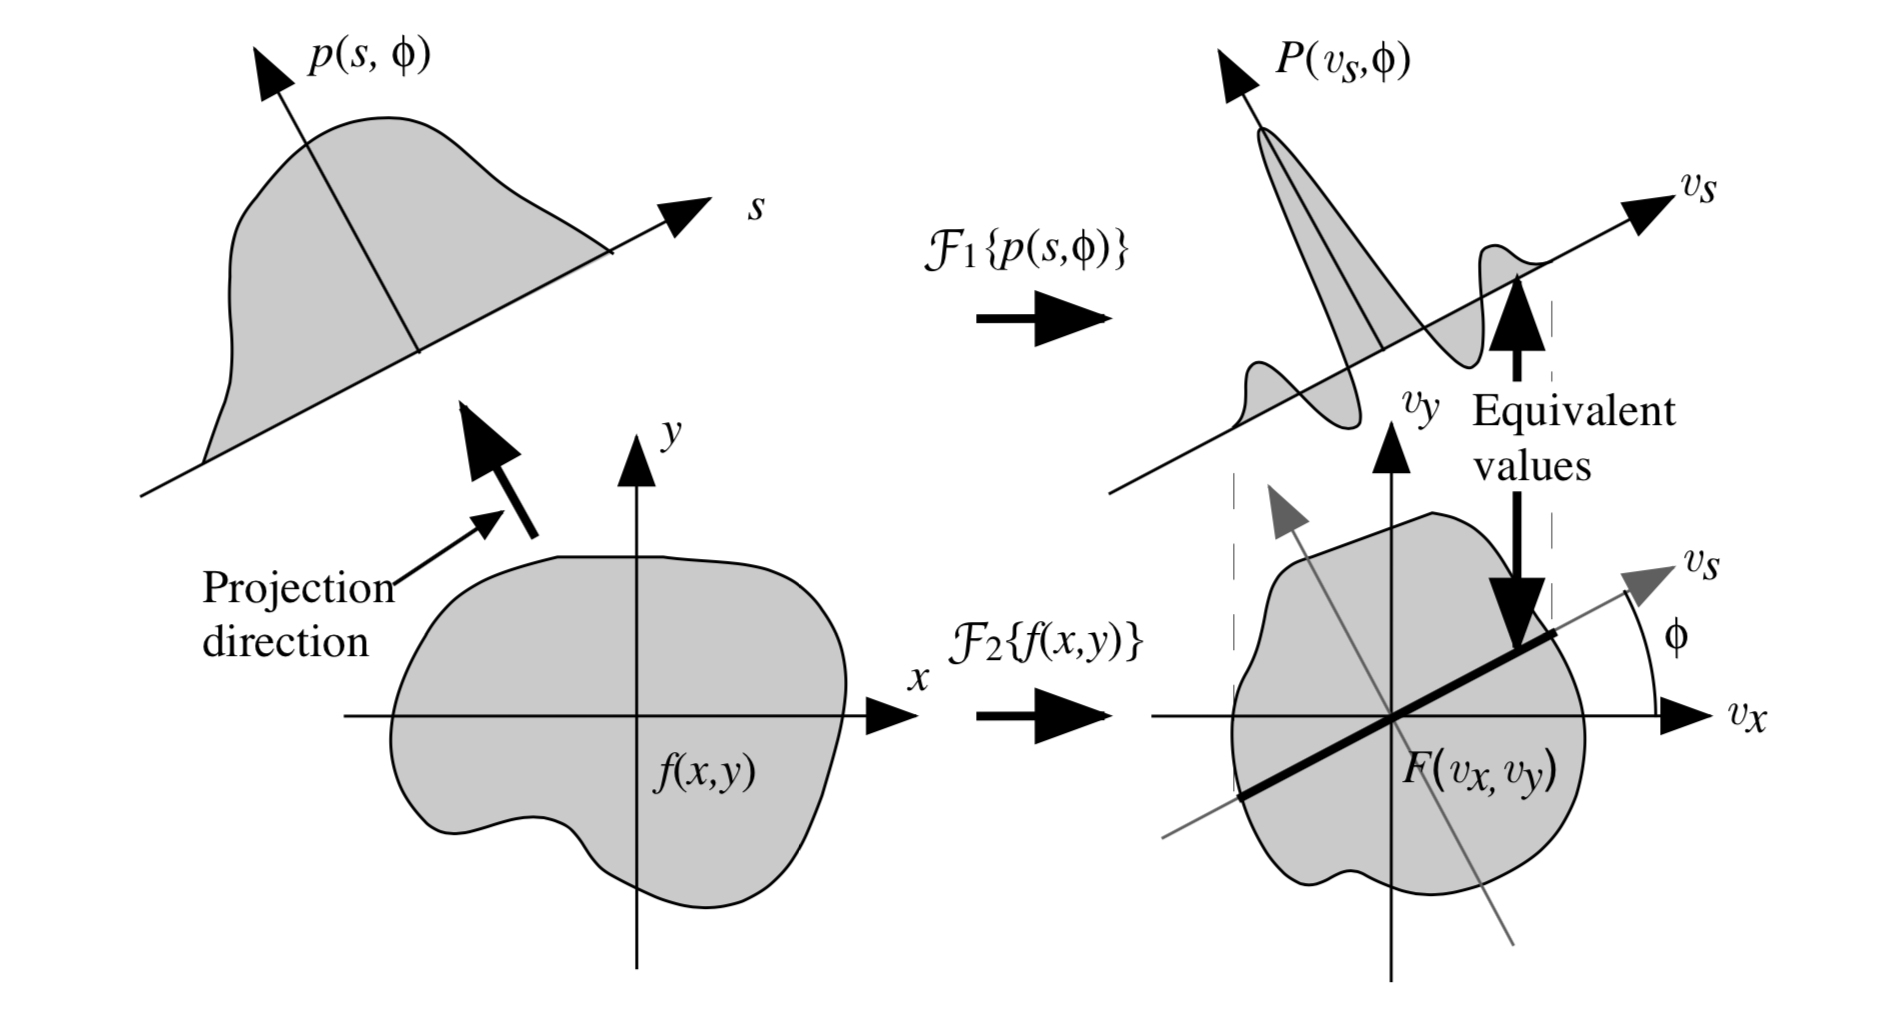
\includegraphics[width=\linewidth]{Background Reading Analysis/Central-section_theorem.png}
    \caption{\label{Fig.Central-Slice}}
\end{figure}

\subsection{Backprojection}
Backprojection is an essential step in image reconstruction. The concept of backprojection involves placing the value of $p(s,\phi)$ along the path of the respective LORs at angle $\phi$. However, because there is no knowledge as to where along the backprojection the values came from, constant values are backprojected along the LOR. This does not return the image due to oversampling in the center of the Fourier transform. 

For example: if we project back at angles $\phi_1$ and $\phi_2$ and examine the result after Fourier, we will see the contribution at the origin is double while there is only one contribution at the edges of the FOV. 
Another example: consider a single point source at the origin, the area around the origin in the reconstructed image will be heavily blurred due to the projections are added back to the entire LOR. These examples of oversampling indicate that some thing needs to be re-weighted/ filtered to obtain equal contributions. 

We can filter the Fourier transform with filter $v = \sqrt{v_x^2 + v_y^2}$ such that the Fourier transform from the backprojection $B(v_x,v_y)$ becomes:

\begin{equation} \label{eq.filtered fourier}
    F(v_x,v_y)= v B(v_x,v_y)
\end{equation}



This desensitizes the Fourier transform with a 'cone' filter. This process is know as \textbf{Backprojection Filtering (BPF)}

\subsection{Filtered Backprojection}
The filtered backprojection equation can be written as:
 \begin{equation} \label{eq.filtered backprojection}
  f(x,y) = \int_0^\pi p^F(s,\phi) d\phi
 \end{equation}
where the filtered projection is given by:
\begin{equation}
	p^F(s,\phi) = \mathcal{F}_1^{-1} \bigg\{ |v_s| \mathcal{F}_1\{ p(s,\phi)\}\bigg\}
\end{equation}
This is 'pre'-corrected for the oversampling of the Fourier transform of $f(x,y)$. 

\subsection{Regularization}
The inverse problem of Eq.\ref{eq.model} (and solving for $f$) is ill-posed and its solution Eq.\ref{eq.filtered backprojection} is unstable in the sense that a small perturbation of the data $p(s,\phi)$ can lead to unpredictable changes in the estimation of $f(x,y)$. Photon detection is stochastic and so regularization can be used to constrain the solution space to physically acceptable values.

We can add a regularization term into the \textbf{FBP} algorithm Eq.\ref{eq.filtered backprojection}:

\begin{equation} \label{eq.apodizing}
	f(x,y) \approx\tilde{f}(x,y) = \int_0^\pi \mathcal{F}_1 \big \{W(v_s) |v_s| \mathcal{F}_1 \{p(s,\phi)\}\big\}
\end{equation}
where $W(v_s)$ is a regularization/ apodizing function.
NOTE: the term "filter" in the literature is reserved for the unique "ramp" filter $|v_s|$ in tomographic image reconstruction.

\subsection{3D image reconstruction}

Two major differences between 2D and 3D image reconstruction are: 
\begin{itemize}
\item Spatially-varying scanner response - In full 3D the scanner is more sensitive to activity at the center of the axial FOV than at the edges. This is because more oblique planes intersect the center of the scanner leading to spatial variance which complicates the image reconstruction.
\item Data Redundancy - Positively - full 3D data contains redundancies due to only a single slice being required, to reconstruct an image, therefore multiple slices of the 3D data are redundant.
\end{itemize}

Spatial invariance of 3D projection data is to use a 3D re-projection algorithm. These algorithms estimate the unmeasured regions of projection by numerically forward-projecting though and estimate image. The inital estiamate is formed from reconstructing an image using only the direct planes (not truncated) with 2D FBP for each transverse plane.

\subsubsection{Rebinning}
3D x-ray transform data can be estimate a stacked (volumetric) set of 2D transverse sinograms by using signal averaging. This is known as rebinning. Each rebinning sinogram can be reconstructed with either analytic or iterative 2D reconstruction methods.
However, there is a price to pay with a penalty in spatially-varying distortion and/or amplification of noise.

Algorithms
Single-slice rebinning (SSRB) is the simplest rebinning algorithm - rebinned sinograms are formed from averaging all of the oblique sinograms that intersect the direct plane at the center of the transaxial FOV.
The Fourier rebinning (FORE) algorithm - based on  reasonably accurate equivalence between specific elements in the Fourier transformed oblique and the transverse sinograms. After normalization of for the sampling of the Fourier transform, sinograms can be recovered from the inverse transform. 
FORE amplifies statistical noise slightly over SSRB but has less distortion. 

\subsection{Iterative Image Reconstruction}

Five Basic Components

1) \textbf{Model for the image} - ie discretization of the image domain into N pixels/ 2D elements or voxels/ 3D elements

2) \textbf{Model for the system} - relate the image to the data. An element $H_{ij}$ of the system model, $\textbf{H}$ characterized the imaging system and represents the probability that an emission from voxel $j$ is detected in projection $i$. $\bar{p}_i = \sum_{j=1}^{N} H_{ij}f_j $ - where $\bar{p}_i$ is the mean of the $i^{th}$ projection and $f_j$ is the activity in voxel $j$.

3) \textbf{Model for the data} - the statistical methods describing the relationship between the value of the measurements and the expected value of the measurement. In other words - this model relates how the projection measurements vary around their expected mean values and is derived from the basic understanding of the acquisition process. Photon detection's are a Poisson distribution so this model is often used. For $M$ projections, the Poisson probability law states that the probably $\textbf{L}$ that the random vector of Poisson distributed photon counts $P$ equals the true photon counts $p$ given we have a vector of emission rates, $f$
\begin{equation}
	\textbf{L}(P=p|f) = \prod_{i=1}^M \frac{\bar{p}_i^{p_i}  e^{-\bar{p}_i}}{p_i!}
\end{equation}
If we correct for things like randoms, scatter, and attenuation, the data is no longer Poisson.
4) \textbf{Governing Principle} - Need to define the 'best' image. This is often mathematically expressed at a cost or objective function. The most common principle for iterative reconstruction is the Maximum Likelihood approach - a standard statistical estimation method which is a probability relationship. We chose an estimate of the object $\hat{f}$ that provides the greatest value of $\textbf{L}$().

Maximum-likelihood estimators are advantageous because the offer unbiased, minimum variance estimates as the number of estimates increases towards infinity. These estimators are proven to provide the least variance among all possible unbiased estimators with less noise than unbiased estimators. Due to the nature of ET and photon emission counting, the noise levels of an unbiased estimator is unacceptable so image reconstruction methods often allow some bias. This bias can be in the form of spatial smoothing - effectively adding error to the image mean values while reducing overall noise levels. This smoothing is performed either by implicitly stopping the algorithm before reaching the ML solution or explicitly through some smoothing operation (i.e. post-processing low-pass filter)

5) \textbf{An Algorithm} to optimize the cost function - Numerous algorithms have been proposed ranging from gradient decent to the more commonly used expectation maximization (EM) algorithm. A variant of this EM algorithm is the Ordered-Subsets Expectation Maximization - which is the most widely used method. 

\subsubsection{Maximum Likelihood - Expectation Maximization}
If our current ($n^{th}$) estimate of voxel $j$ is $\hat{f}^{(n)}_j$ then our future estimate will be $\hat{f}^{(n+1)}_j$

(NOTE: The next equations are generated in steps)

Forward project on all $k$ projections:
\begin{equation}
	\sum_k H_{ik} \hat{f}_k ^{(n)}
\end{equation}
Compare these estimate projections with measured projections to form a multiplicative correction factor for each projection:
\begin{equation}
	\frac{p_i}{\sum_k H_{ik} \hat{f}_k ^{(n)}}
\end{equation}
Back-project these ratios (into the image domain) to obtain a correction factor for the initial estimate:
\begin{equation}
	\sum_i H_{ij}\frac{p_i}{\sum_k H_{ik} \hat{f}_k ^{(n)}}
\end{equation}
Multiply the current image estimate by the correction estimate and divide by a weighting term based upon the system model to apply the desired strength of each image correction factor:
\begin{equation}
	\hat{f}_j^{(n+1)} = \frac{\hat{f}_j^{(n)}}{\sum_{i'} H_{i'j}}\sum_i H_{ij}\frac{p_i}{\sum_k H_{ik} \hat{f}_k ^{(n)}}
    \label{eq.ML-EMiteration}
\end{equation}
The algorithm now recenter the new estimate $\hat{f}_j^{(n+1)}$ as the new estimate and repeats.

As the EM algorithm iterative guesses an image estimate, low frequency components appear in a few iterations. As the ML estimate is approached, higher frequency  definition is resolved in the image - effectively adding more variance to the reconstructed image. As previously mentioned, the variance can be reduced with early-stopping or by post-smoothing the reconstruction. 

While the convergence rate of the image reconstruction is image dependant, it typically takes between 20 and 50 iterations to reach an acceptable solution. Considering the ML-EM algorithm requires a forward and backward  projection at each iteration, the overall processing time is much greater than that of the filtered backprojection approach aforementioned but leads to a potentially more accurate reconstruction. 

\subsubsection{Ordered Subsets Expectation Maximization (OSEM)}
Aims to reduced reconstruction time of conventional ML-EM by breaking the data into subsets.
\begin{equation}
	\hat{f}_j^{(n+1)} = \frac{\hat{f}_j^{(n)}}{\sum_{i'\in S_b} H_{i'j}}\sum_{i \in S_b} H_{ij}\frac{p_i}{\sum_k H_{ik} \hat{f}_k ^{(n)}}
    \label{eq.OSEMiteration}
\end{equation}
This image update algorithm only differs to ML-EM via the backprojection steps sum over the projections in a subset $S_b$ in a total of $B$ subsets. An image is updated after $B$ sub-iterations as each of the subsets are iterated. If $B=1$ then OSML is the same as ML-EM.

There are different approaches for organization of projection space subsets.


\subsection{Bayesian/Penalized Methods}
Bayesian methods attempt to improve image quality by taking advantage of knowledge of the image:
\begin{itemize}
\item non-negative tracer concentrations
\item only small variation between neighboring voxels
\end{itemize}
This information is known \textit{a priori} and using Bayes' Rule, is often incorporated into a maximum \textit{a posteriori} (MAP) objective function. This objective function includes all the available information after the reception of \textit{a priori} knowledge of the image.

On the basic level, the image estimates in the iterative process are a "prior" term and leads to the guarantee of convergence with certain algorithms. Therefore, these methods are equivalent to using a "penalty" term at each iteration and these methods are also termed penalized.

The prior penalty term can promote desired properties in the image such as smoothness, edges, or even particular structure based upon anatomical information from separate CT/MR studies.

One significant challenge when applying prior/penalty terms is choosing a strength parameter that varies the influence, or strength, the penalty will have on the image. 

This leads to more complex implementation and although these Bayesian methods are starting to see clinical implementation, they are slow to uptake these methods due to the challenge of choosing an appropriate parameter for governing the strength of the penalty term.


\subsection{3D Iterative Reconstruction}

Conceptually, the same iterative methods can be extended to fully 3D PET measurements and reconstruction as previously mentioned for the 2D images. The difference is the image model is now a 3D volume with voxels instead of a 2D image with pixels.

The primary challenge for 3D PET reconstruction is the major increase in computational demand. 
\begin{itemize}
\item The image sizes increase from $10^4$ pixels to $10^5$ voxels.
\item The dataset increases from $10^4$ to as much as $10^7$ entries. 
\item The system model must be computed for effectively $10^{12}$ combinations (instead of $10^8$ for 2D PET)
\end{itemize}
A further option for the iterative methods is to first re-bin the 3D data into 2D transaxial slices (as aforementioned) then proceed with the faster 2D iterative reconstruction processes.

\subsection{Definitions of Image Quality}
There is a challenge in tomographic reconstruction techniques - which method of reconstruction provides the 'best' image. Two of the major imaging task categories are classification tasks and estimation tasks. Classification tasks categorize the image or features in the image into one or more classes. A common classification task is detection (a binary classification task). Some other examples of classification tasks include signal detection, image segmentation, and diagnosis. On the other hand, estimation tasks seek numerical parameters from an imaging system such as the quantitation of physiological parameters or the estimation of features for pattern recognition. Specific examples of estimation tasks include a cardiac ejection fraction or the value of tracer flux in a tissue compartment model.

One common approach to assess image quality is to look at figures of merit  such as: signal to noise ratio, bias, contrast levels etc. However care must be taken when assessing these measures as the image volume of $10^6$ elements is described by just a few descriptor values. 

Another trade-off is in image quality is bias vs. variance. PET data is random - meaning if you imaged the same object multiple times, the reconstructed images would differ due to statistical variations in the model. We would prefer to have a reconstruction method which creates an image that is on average the true image: an unbiased method. That being said, we would prefer a reconstruction method that creates and image whose values do not deviate from their mean values: a zero variance method.
\begin{itemize}
\item Bais is a measure of the accuracy of our reconstruction on average
\item Variance is a measure of the precision of the estimate.
\item Thank to the target board example.
\end{itemize}


\newpage
\section{Nuclear Medicine Physics: A Handbook for Teachers and Students} \cite{Bailey2014}

\subsection{Chapter 13: Image Reconstruction}
This is known as an inverse problem - it is harder to make software to compute the true tracer distribution from photon data than to simulate tracer distribution and predict photon acquisition. As other books have mentioned, there are really two ways to reconstruct and image - analytically using mathematical inversion and iterative...


Central slice/section theorem is important in analytically reconstruction as it gives the relationship between the Fourier transform of an image and its parallel projections.

\textbf{Radon (x-ray) Transform}

\begin{equation}
\begin{split}
	Y(s,\phi) & = \int_{-\infty}^{\infty} \int_{-\infty}^{\infty} \Lambda (x,y) \delta_{s=x\cos\phi + y\sin\phi}\ dx\ dy\\
   & =\int_{-\infty}^\infty \Lambda (s\cos\phi - t\sin\phi, s\sin\phi + t\cos\phi)\ dx\ dy
    \label{eq.x-ray transform}
 \end{split}
\end{equation}	
Where $\delta$ is unity for the points on the LOR $(s,\phi)$ and zero everywhere else. The Radon Transform describes the acquisition process in 2D PET and SPECT (with parallel hole collimation and attenuation ignored).

\textbf{Backprojection}
\begin{equation}
\begin{split}
B(x,y) &= backproj(Y(s,\phi)) \\
& =\int_0^\pi d\phi \int_{-\infty}^{\infty} Y(s,\phi)\delta_{s=x\cos\phi + y\sin\phi}\ ds \\
& = \int_0^\pi Y(x\cos\phi + y\sin\phi, \phi) d\phi
\end{split}
\end{equation}
NOTE This backprojection is not the inverse of the projection, $B(x,y) \neq \Lambda(x,y)$ 

The central slice theorem used to reconstruct an unknown image Λ(x, y) from its known projections y(s, φ).




The FBP algorithm. This algorithm involves the following steps:

\begin{enumerate}
\item apply 1-d Fourier transform to $Y(s, φ)$ to obtain $(\mathscr{F}_1y)(ν, \phi)$;
\item filter $(\mathscr{F}_1y)(ν, \phi)$ with the so-called ramp filter $|ν|$;
\item apply the 1-D inverse Fourier transform to obtain t:/he ramp filtered projections $\hat{Y}(s,\phi) = \int \mathscr{F}_1 Y(\nu, \phi) |v| e^{i2\pi\nu s}d\nu$
\item apply the back-projection operator eq.(13.2) to $Y(s,\phi)$ to obtain the desired image Λ(x, y).
\end{enumerate}


\subsubsection{Iterative Reconstruction}
In analytically reconstruction, it is initially assumed that the unknown object can be represented as a function $\Lambda(\vec{x}),\ \vec{x}\in \mathbb{R}^3$ and data is acquired as a function $Y(s,\theta), s\in\mathbb{R}^2$ and $\theta$ a unit vector in $\mathbb{R}^2$ or $\mathbb{R}^3$. The reconstruction algorithm is then derived via mathematical inversion resulting in a algorithm that is discretized for software implementation.

In iterative reconstruction, the problem is initial discretized to reduce the reconstruction problem to finding an finite set of unknown values from a finite set of equations, which can be numerically solved. The advantage of numerical inversion is that only a model for the acquisition process is needed, not for its inverse. That makes it easier (although it may still be non-trivial) to take into account some of the undesired but unavoidable effects that complicate the acquisition, such as photon attenuation, position dependent resolution, gaps between the detectors and patient motion.

We call the unknown image values $\lambda$ and the known measured values $\textbf{y}$. The image can be reconstructed with:

\begin{equation}
\textbf{y} = \textbf{A} \lambda +\bar{\textbf{b}} +\textbf{n}
\end{equation}
where $\bar{\textbf{b}}$ is some additive contribution and $\textbf{n}$ is measurement noise. This can be written in element form
\begin{equation}
y_i = \sum_{j=1}^J = A_{ij}\lambda_{j} +\bar{b}_j + n_j, \ \ \ \ \ \ i=1,...,I 
\end{equation}
Here $y_i$ denotes the number of photons measured on the $i^{th}$ LOR, where $i$ runs over all the sinogram elements. $j$ runs over all the image voxels. $A_{ij}$ is the probability that a unit of radioactivity in $j$ gives rise to the detection of a photon pair (PET) in the $i^{th}$ LOR. $\bar{\textbf{b}}$ represents the background noise i.e. scatter and randoms in PET. Finally we have $n_i$ that represents the noise contribution to the $i^{th}$ LOR. 

So basically, find $\lambda$ given $\textbf{A},\textbf{y},\bar{\textbf{b}}$ and a statically noise model for $\textbf{n}$. 

\textbf{Objective functions}

The presence of noise precludes exact reconstruction and thus reconstruction is viewed as an optimisation task.

We can apply a Bayesian approach by searching for an image $\hat{\lambda}$ that maximises the conditional probability on the data.

\begin{equation}
\begin{split}
\hat{\lambda} &= \text{argmax} \ P(\lambda|\textbf{y}) \\ 
&= \text{argmax} \ \frac{P(\textbf{y}|\lambda)P(\lambda)}{P(\textbf{y})} \\
&= \text{argmax} \ P(\textbf{y}|\lambda)P(\lambda)\\
&= \text{argmax} (\ln{\text{argmax} \ P(\textbf{y}|\lambda)}  + \ln{P(\lambda)}  )
\end{split}
\end{equation}
the second equation is Bayes' Rule, the third equation holds because $\textbf{y}$ does not depend on $\lambda$, and the fourth is valid because a logarithm does not change the position f the maximum.

The probability $P(\textbf{y}|\lambda)$ is the likelihood of measuring the sinogram $\textbf{y}$ if the tracer distribution is $\lambda$. The probability $P(\lambda)$, often know as the prior distribution, represents a priori knowledge of the tracer distribution available before PET acquisition.
 
 \subsubsection{\textbf{Optimisation algorithms - Page 473}}
The objective function:
\begin{equation}
\hat{y}_i = \sum_i A_{ij}\lambda_j  \bar{b}
\end{equation}
is considered optimised when its first derivatives are zero

\begin{equation}
\frac{\delta L_{ML}(\lambda)}{\delta\lambda_j}=\sum_i A_{ij} \frac{y_i - \hat{y}_i}{\hat{y}_i} 
\end{equation}
 The optimisation can be carried out by a steepest ascent method. The gradient of the previous objective function:
 \begin{equation}
 \textbf{d}^k= \nabla  L(\lambda^{k-1})
 \end{equation}
 Increments the update of the object:
 \begin{equation}
 \lambda^k = \lambda^{k-1} +a_k \textbf{d}^k
 \end{equation}
 where the multiplier $a_k$is given by:
\begin{equation}
a_k = \text{arg max} L(\lambda^{k-1} +\alpha\textbf{d}^k )
\end{equation}
Where k and k-1 represent the iteration number and $\nabla L$ represents the vector of the first derivatives of \textit{L} w.r.t. $\lambda_j$.

This method of steepest gradient ascent is known to be sub-optimal, requiring multiple iterations to reach a reasonable convergence. Approximate the first derivatives if $L$ with the first order Taylor Expansion gives:
\begin{equation}
\nabla L(\lambda^{k-1} + \textbf{p}_k ) = 0
\end{equation}
\begin{equation}
\nabla L(\lambda^{k-1}) + \textbf{H}\textbf{p}_k \approx  0
\end{equation}

\begin{equation}
\begin{split}
\textbf{p}_k &= -\textbf{H}^{-1} \nabla L(\lambda^{k-1}) \\
&= \textbf{H}^{-1} \textbf{d}^k
\end{split}
\end{equation}

\textbf{p}_k = -$\textbf{H}$ is the Hessian (second order derivatives of $L$). This matrix is very large but easy to compute for the weighted least squared (WLS) and Maximum Likelihood (ML) objective functions. It is usually impossible to calculate the inverse of $\textbf{H}$. Instead, other algorithms can be used to obtain a good $\textbf{M}$ do derive a so-called preconditioned gradient acent algorithm:
\begin{equation}
\begin{split}
& \textbf{d}^k = \nabla L(\lambda^{k-1})\\
& \lambda^k = \lambda^{k-1} + \alpha_k \textbf{M}\textbf{d}_k
\end{split}
\end{equation}
It should be noted that $\textbf{M}$ must be symmetric positive definite to ensure convergence. A simple way to obtain a reasonable $\textbf{M}$ is to use only the diagonal elements of $\textbf{H}$: $\textbf{M}_{ii} = –1/\textbf{H}_{ii} \text{ and } \textbf{M}_{ij} = 0 \text{ if } i \neq j$. However, there are other more sophisticated methods and this optimisation function is used.

In every iteration, the algorithm starts moving in the direction of maximum gradient (i.e. perpendicular to the isocontour)  and keeps moving along the same line until a maximum is reached (i.e. the line is tangent to the isocontour). This will often lead to a zigzag line, see Fig.\ref{Fig.isocontourzigzag}.
\begin{figure}
\centering
	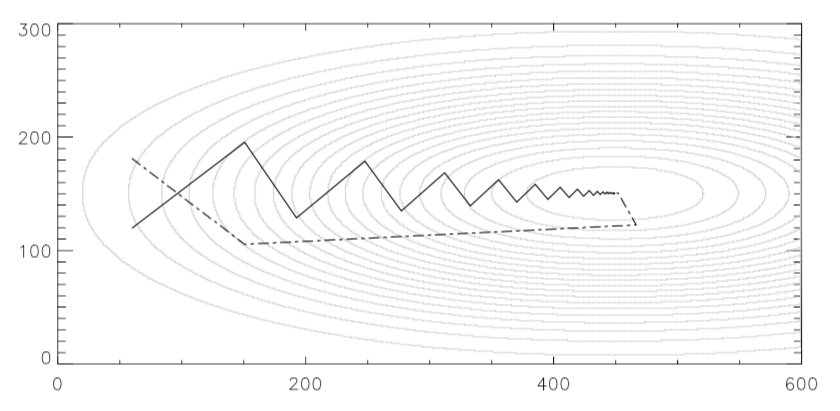
\includegraphics[width=\linewidth]{Background Reading Analysis/IsocontourZigZag.png}
    \caption{\label{Fig.isocontourzigzag}}
\end{figure}





\\subsubsection{Maximum -likelihood expectation-maximisation (MLEM)}
We with to find the image $\lambda$ that maximises the likelihood function $L_{ML}$. \textbf{EM} does this differently. Instead of concentrating on $L_{ML}$, \textbf{EM} introduces a set of so-called '\textit{complete data}' $x_{ij}$, defined as the number of photons that were emitted from voxel $j$ and detected along LOR $i$ during measurement. This unobserved data are 'complete' in the sense they describe more detail than the observed data $y_i$ (the measurements). The variables $x_{ij}$ are Poisson distributed. We can write the log-likelihood function for observing the data $x_{ij}$ are while $\bar{x}_{ij} = A_{ij}\lambda_j$ were expected:

\begin{equation} \label{eq.log-likelihood_x}
L_x(\lambda) = \sum_i \sum_j x_{ij} \ln (A_{ij} \lambda_j) - A_{ij}\lambda_j
\end{equation}
However this cannot be computed because the data $x_{ij}$ are not available. The emission measurement only produces the sum of the complete data, since:
\begin{equation} \label{eq.project_x}
y_i = \sum_j A_{ij} x_{ij} + b_i
\end{equation}
where $b_i$ represents the actual (also unobserved) additive contribution $b_i$ in LOR $i$.

The \textbf{EM} recipe prescribes computing the expectation of $L_x$ based on the available data and the current reconstruction. Based on the reconstruction alone, the estimate would be written as:
\begin{equation}
E(x_{ij}|\lambda^{(k)}) = A_{ij}\lambda_j^{(k)}
\end{equation}
However, as we know that $x_{ij}$ should satisfy Eq.\ref{eq.project_x}  the estimate becomes:
\begin{equation}
E(x_{ij}|\lambda^{(k)},\textbf{y}) =  \frac{y_i}{\sum_j A_{ij}\lambda_j^{(k)} + \bar{b_i}}    A_{ij}\lambda_j^{(k)}
\end{equation}

Inserting this equation into the log-likelihood expression for $L_x(\lambda)$ Eq.\ref{eq.log-likelihood_x} completes the expectation (E) step. Maximisation occurs when the derivative is set to zero.

\begin{equation} \label{eq.LikelihoodGradient}
\frac{\delta L_x(\lambda)}{\delta\lambda_j} = \sum_i \bigg( \frac{y_i}{\sum_j A_{ij}\lambda_j^{(k)} + \bar{b}_i}\bigg) A_{ij}\lambda_j^{(k)} \frac{1}{\lambda_j} - A_{ij}\bigg)  = 0
\end{equation}
This is easily solved for $\lambda_j$ yielding a new reconstruction of $\lambda_j ^{(k+1)}$ .
\begin{equation}\label{eq.MLEM equation}
\lambda_j ^{(k+1)} = \frac{\lambda_j ^{(k)}}{\sum_i A_{ij}}\sum_i A_{ij}\frac{y_i}{\sum_j A_{ij}\lambda_k^{(k)}+\bar{b}_i}
\end{equation}
This is the well known MLEM algorithm for emission tomography. Each iteration of this raises the value of the likelihood $L_{ML}$. The complete data $x_{ij}$ does not appear in \ref{eq.MLEM equation} but is needed within the derivation. The initial image $\lambda^{(0)}$ must be provided given the iterative algorithm. Typically a uniform positive image is chosen. 

The MLEM algorithm is multiplicative and so the voxel values must be non-zero to be updated. Additionally, the voxel values should be non-negative to avoid a divergent model. Sometime prior operations can lead to negative values and these will likely lead to a divergent system.

\subsubsection{Regularisation}
MLEM maximises the likelihood by making computed projections as similar as possible to the measured projections, where the similarity is measured based on the Poisson distribution. An upper limit of the  likelihood would be obtained when the measured and calculated projections are identical. However, this is never possible, because Poisson noise introduces inconsistencies. However, most of the noise is consistent and so it propagates through the iterations into the reconstructed image leading to the deterioration of the MLEM image at high iteration numbers.

\textbf{Maximum a posteriori or Penalised likelihood}
Smoothing the MLEM image is not elegant, first the likelihood is maximised and then decreased by smoothing the image. A more sophisticated method would be to modify the objective function. This can be done using a Bayesian approach, equivalent to combining the likelihood with a penalty function.

It is assumed that a good reconstruction image $\lambda$ will be obtrained if that image maximises the (log of the) probability $p(\lambda|\textbf{y})$ given:

\begin{equation}
\hat{\lambda} = \text{arg max} \ln p(\lambda|\textbf{y}) + \ln p(\lambda)
\end{equation}
The second term represents the priori knowledge about tracer distribution, which we usually believe is smooth. This is achieved with a Markov prior that governs the probability for a particular voxel, given the value of other voxels in it's neighbourhood $\textbf{N}_j$. Such priors are usually written in the following form:
\begin{equation}
\begin{split}
P(\lambda) 
&= \ln p(\lambda)\\
&= \sum_j \ln p(\lambda_j | \lambda_k , k\in \textbf{N}_j)\\
&= -\beta \sum_j \sum_{k\in \textbf{N}_j} E(\lambda_j, \lambda_k)
\end{split}
\end{equation}
where $E(\lambda_j \lambda_k)$ an 'energy' function designed to obtain noise suppressing behaviour and the parameter $\beta$ is the weight assigned to the prior information.
There are many possible energy functions but generally they further simplify the function by taking the absolute difference of the voxels $x =|\lambda_j - \lambda_k|$. Some popular energy functions are: quadratic $x^2$, Huber prior (quadratic for $x \leq 1$ and linear for $x \gt 1$), and Geman, which converges asymptotically for a constant of large differences, implying it does not smooth for all over very large pixel differences. 

It can be shown, if $E(\lambda_j \lambda_k)$ is concave then the system is concave with one maxima, i.e. the quadratic and Huber energy functions. In contrast, the Geman is not concave and so can result in local maxima leading to careful initialisation of the iterative method because the final image depends on the starting location.

When MAP (maximum a posteriori) with a quadratic prior reconstructs with position dependant smoothing due to the likelihood being reduced with less photons as a result of photon attenuation.

\subsubsection{One Step Late}
An example of a MAP algorithm involves adding of the derivitive of prior $P(\lambda)$ to Eq.\ref{eq.LikelihoodGradient}.

\begin{equation} \label{eq.OneStepLate}
\begin{split}
\frac{\delta( L_x(\lambda) + P(\lambda))}{\delta\lambda_j} & = \sum_i \bigg( \frac{y_i}{\sum_j A_{ij}\lambda_j^{(k)} + \bar{b}_i}\bigg) A_{ij}\lambda_j^{(k)} \frac{1}{\lambda_j} - A_{ij}\bigg)  + \frac{\delta P(\lambda)}{\delta \lambda_j} \\
&= \sum_i \bigg( \frac{y_i}{\hat{y}_i^{(k)}}\bigg) A_{ij}\lambda_j^{(k)} \frac{1}{\lambda_j} - A_{ij}\bigg)  + \frac{\delta P(\lambda)}{\delta \lambda_j}\\
&= 0
\end{split}
\end{equation}
The issue with this equation is the derivative $\frac{\delta P(\lambda)}{\delta \lambda_j}$ is a function of the unknown image so we must use the current reconstruction$\lambda^{(k)}$ so the updated image can be given by:

\begin{equation}
\lambda_j^{(k+1)} = \frac{\lambda_j^{(k)}}{ \sum_i A_{ij} - \frac{\delta P(\lambda)}{\delta \lambda_j}\bigg|_{\lambda^{(k)}} }  \sum_i A_{ij} \frac{y_i}{\hat{y}_i^{(k)}}
\end{equation}
\subsubsection{Corrections for distortions and contamination of physical effects}
Types distortion effects:

\begin{itemize}
\item detector resolution 
\item collimator effects
\item non-collinearity  
\item positron range) 
\item motion effects
\end{itemize}

The contamination effects can be divided into multiplicative and additive terms. 
The multiplicative factors include: 
\begin{itemize}
\item attenuation
\item detector normalisation factors
\item coefficients accounting for the decay time
\item geometrical restriction
\end{itemize}
The additive terms include: scattered and random coincidences.

The easiest approach to compensate for the contamination effects is to include a multiplicative correction term to the system model while preserving the Poisson characteristics of the data. However, this can lead to an increase in the number of non-zero elements of the system matrix (i.e. the matrix is no longer sparse) and thus the system is more ill-posed and thus more computationally expensive.

The more commonly used and practical approach is to use correction effects as multiplicative factors and additive terms within the forward projection of the model for the iterative reconstruction algorithms:

\begin{equation}
\textbf{y} = \textbf{A}\lambda+\textbf{b}
\end{equation}
Here the corrections are applied within the system matrix $\textbf{A}$  

\textbf{Multiplicative effects}
We can factor the system matrix into its multiplicative components:
\begin{equation}
\textbf{A} = \textbf{A}_{det.sens}\textbf{A}_{det.blur}\textbf{A}_{att}\textbf{A}_{geom}\textbf{A}_{tof}\textbf{A}_{positron}
\end{equation}
\begin{itemize}
\item $\textbf{A}_{positron}$ models the positron range
\item $\textbf{A}_{tof}$ models the timing accuracy of the TOF PET systems
\item $\textbf{A}_{geom}$ the geometric projection matrix is the core of the system matrix with geometric mapping between the source (voxel $j$) and data (projector bin $i$, defined by the LOR or time bin in the TOF cases). This does geometrical mapping based on probability (in absence of attenuation) that photon pairs emitted from image location reach the front faces of a given crystal pair (LOR).
\item $\textbf{A}_{att}$ is a diagonal matrix containing attenuation factors on individual LORs
\item $\textbf{A}_{det.blur}$ models the accuracy of reporting the true LOR positions
\item $\textbf{A}_{det.sens}$ a diagonal matrix modelling the probability that an event will be reported once the photon pair reaches the detector surface. This is a unique multiplicative factor for each detector crystal pair (LOR) modelled by normalisation coefficients, but can also include detector axial extent and detector gaps. 

\end{itemize}
\textbf{Additive contributions}
The two major additive contaminators are scatter (in both PET and SPECT) and random events (PET). Simply subtracting the estimates ($\bar{s}$ and $\bar{r}$) from the acquired data works in analytically reconstruction but is not effective in statistical iterative methods. These methods (such as MLEM) are designed for Poisson distributed data and furthermore, subtraction of the estimates may introduce negative values to the pre-corrected data (reminder, iterative methods cannot handle negative values as it leads to a divergent algorithm). 

In practice, these compensation terms are included in the bias of the forward projection \textbf{b} = $\bar{s} +\bar{r}$ miscellaneous






\newpage
\section{Image Reconstruction - a tutorial} \cite{Zeng2001}

2D pictures of a 3D object are the projections. The image reconstruction process takes these projections and tries to determine an image of the object.  

The rest of this document was well covered in Alessio's document \cite{Alessio2006} 








\newpage

\bibliography{ref.bib} 
\bibliographystyle{plain}\bibliographystyle{plain}

\end{document}